The Student-t Latent Variable Model (SPLVM) is based upon the notion that a Student-t process can more accurately fit data with a higher percentage of outliers due to broader flanks. This, in theory resembles a higher volatility, but it is not directly implemented into the model. Overall, expectations are, that the higher robustness towards outliers will improve upon the results of the GPLVM. \newline \newline
First, we implement the model, similar to the GPLVM model, but using a function that solves the model using multivariate Student-t distributions. Compare the model code in Appendix \ref{sec:model_code}. Analyzing the closed form solutions described in \ref{sec:student-t}, we find that the Student-t process will behave like the GPLVM, but with an additional multiplicative term giving more flexibility to the covariance matrix. Also, we observe that a Student-t process will become a Gaussian Process for the degree of freedom parameter $\nu \to \infty$, the evaluation of $\nu$ will be particularly interesting for interpretation. It can solve the question of whether a Gaussian process ($\nu \to \infty$), a Student-t Process ($\nu \in [2,\infty)$) solve the problem best, and even show tendencies since the interval is defined over all possible values for $\nu \in \mathbb{R}_0^+$. A rule of thumb in practice is, that from a value of $\nu \geq 30$ on, the Student-t distribution is sufficiently well approximated by a Gaussian distribution. 
The optimal inferred values of $\nu$ are shown in table \ref{tab:splvm_nu}, for the calculations the same input sizes are used as in the main GPLVM run, $N=120$, $D=754$. 
\begin{table}
    \centering
	\begin{tabular}{||l|r|r|r|r|r|r||}\hline
		$\nu$     & Q1        &  Q2       & Q3        & Q4        & Q5        & Q6        \\ \hline
		lin       &  8.847574 &  2.006339 &  2.001937 &  8.651835 &  2.007558 &  2.002983 \\
		exp       &  2.008647 &  2.003451 &  2.009492 &  2.003444 &  2.003168 &  2.001988 \\
		exp2      &  2.002464 &  2.007803 &  2.002753 &  8.199555 &  2.001955 &  2.009912 \\
		mat32     &  8.351861 &  2.002681 &  2.002718 &  2.003437 &  2.006565 &  2.009912 \\
		mat52     &  2.002612 &  2.011853 &  2.004670 &  2.002371 &  2.003071 &  2.001988 \\ \hline
	\end{tabular}
	\label{tab:splvm_nu}
\end{table}
Therefore, we can conclude temporarily that A more Student-t like stochastic process is probably better suited. We find the results of the Student-t model as figure \ref{fig:studt_ELBO_R2}, further exemplifying the notion that the Student-t process is better suited, if not by much. Again, the same holds as with the GPLVM, where the linear kernel underperforms, and higher numbers of latent dimensions perform better. 
\begin{figure}%fig:studt_ELBO_R2      ELBO/R2 values of SPLVM
	\centering
	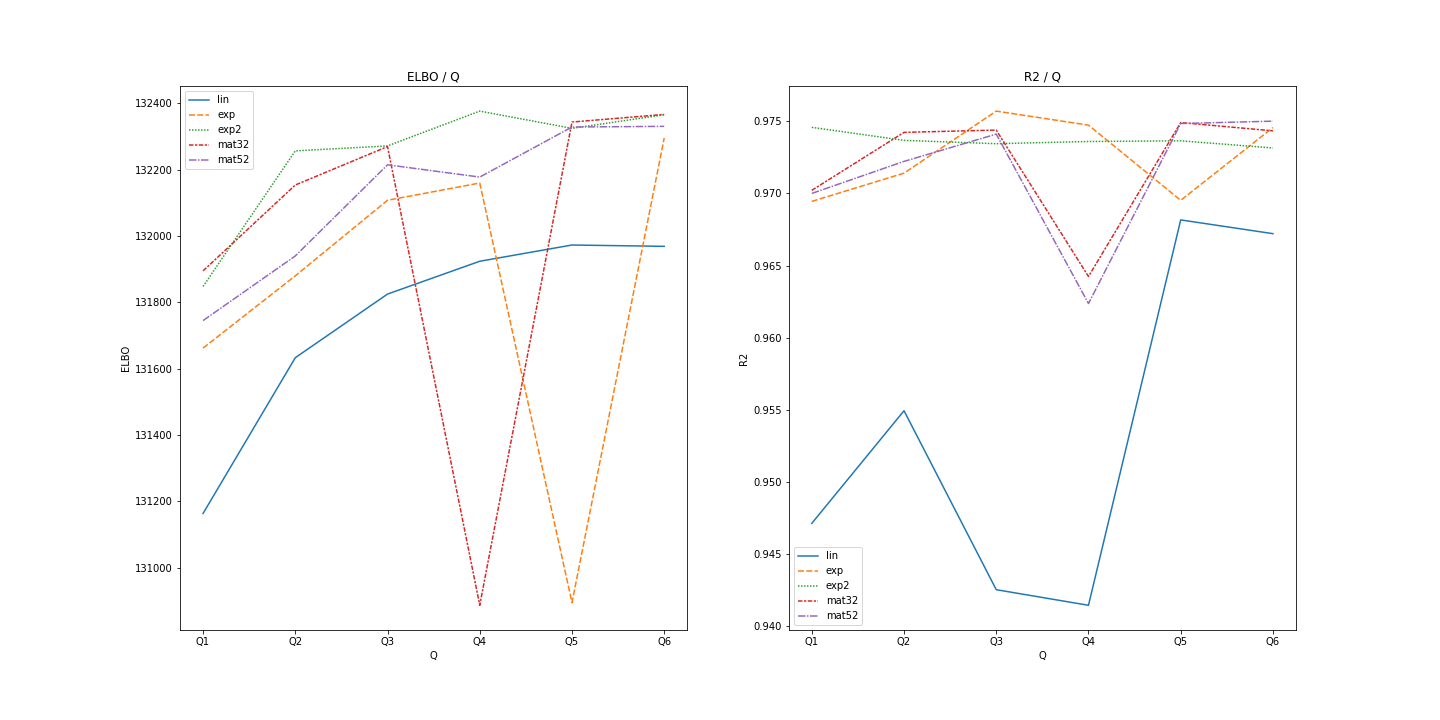
\includegraphics[width=4in]{img/07_1/modelSTUDT_Qs.png}
	\caption[SPLVM ELBO and $R^2$ values for the $N=120$, $D=754$ dataset.]{ELBO and R2 values of the Student-t Process Latent Variable Model (SPLVM).}
	\label{fig:studt_ELBO_R2}
\end{figure}
The distributions of intercept values and slope values of the 120 stocks are shown in figures \ref{fig:studt_intercepts} and \ref{fig:studt_slopes}. Here, we see that the SPLVM model again performs slightly better than the GPLVM. We attribute this performance increase to the broader flanks of the Student-t distribution. Therefore, the outliers seem to be a problem. This does not explain which influences result in those outliers. 
\begin{figure}%fig:studt_intercepts      SPLVM Intercept distributions
	\centering
	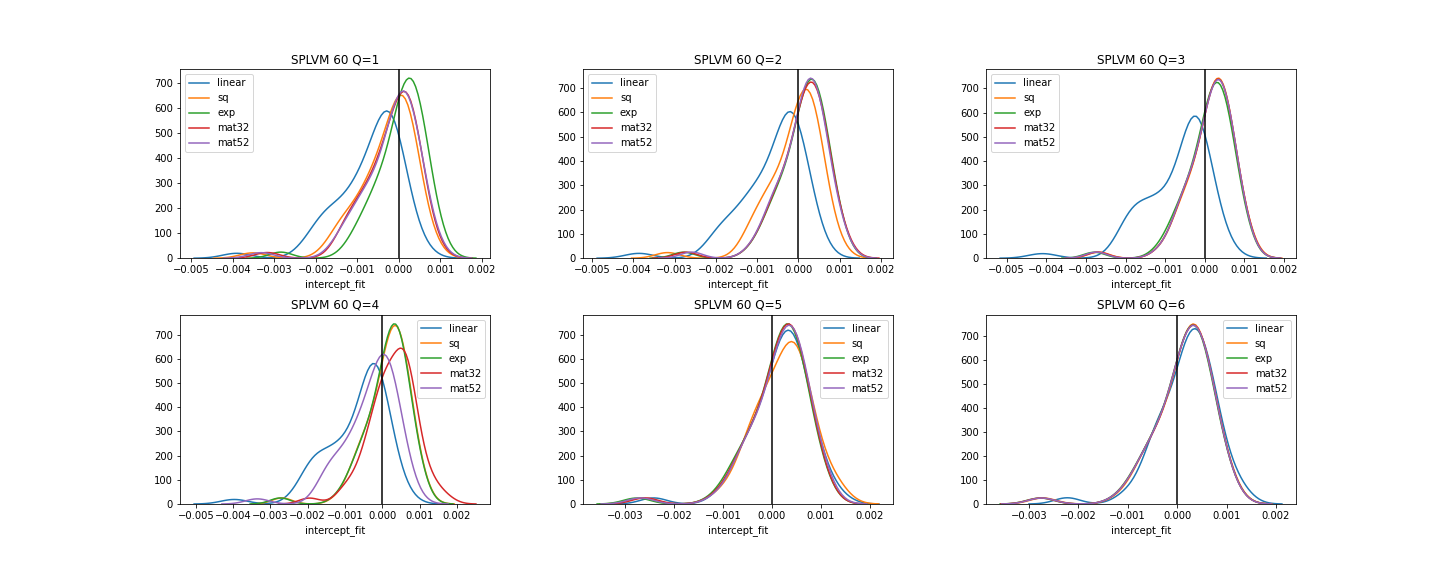
\includegraphics[width=7in]{img/07_1/intercept_fit_studt_120.png}
	\caption[SPLVM intercept values for $N=120$, $D=754$]{The distributions of the intercept values, which should be centered around the vertical line at $x=0$. }
	\label{fig:studt_intercepts}
\end{figure}
\begin{figure}%fig:studt_slopes      SPLVM Slope distributions
	\centering
	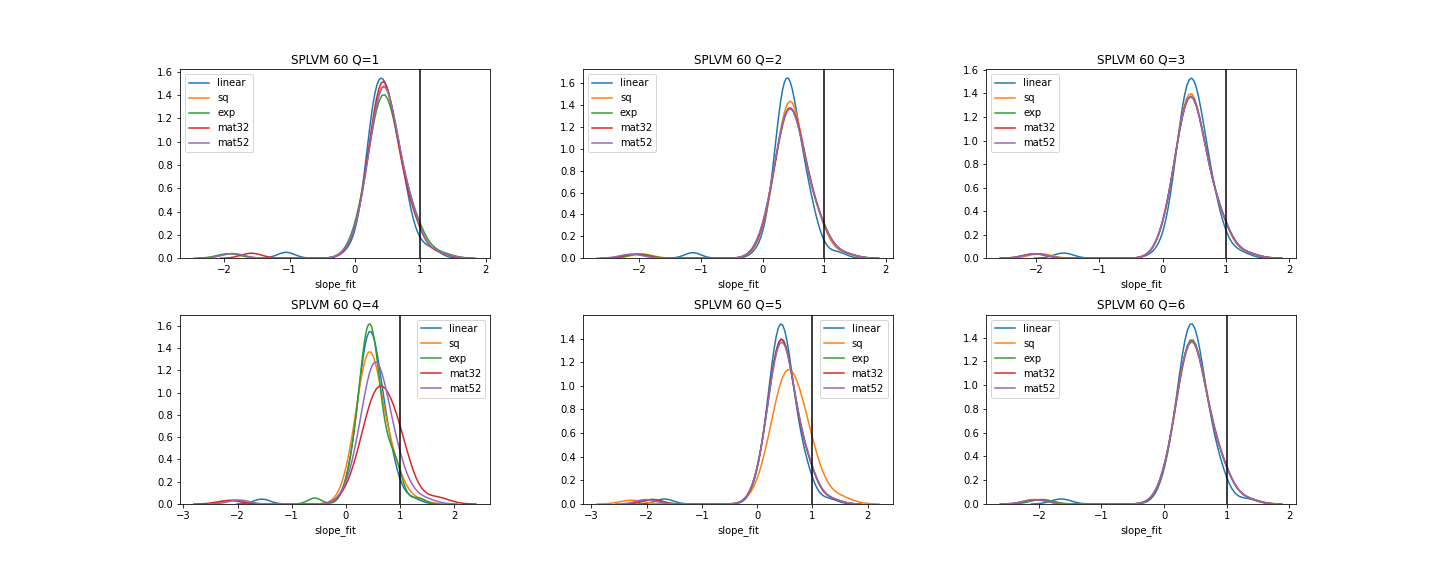
\includegraphics[width=7in]{img/07_1/slope_fit_studt_120.png}
	\caption[SPLVM slope values for $N=120$, $D=754$]{The distributions of the slope values, which should be centered around the left of the vertical line at $x=1$. }
	\label{fig:studt_slopes}
\end{figure}
Just as the GPLVM model, the SPLVM model initializes with any regular data set size, the noticeable difference here, is that it performs so much worse with the VN data sets, that it did not initialize at all. This leads to the assumption, that the volatility does contribute into the broader flanks of the Student-t distribution. Also, we conclude the same sanity checks as before in section \ref{res:gplvm}, looking at the noise and the variance entries. Figures \ref{fig:studt_noises} and \ref{fig:studt_variances} show that for all models, the noise and variance entries show no erroneous behavior. 
\begin{figure}%fig:studt_noises
	\centering
	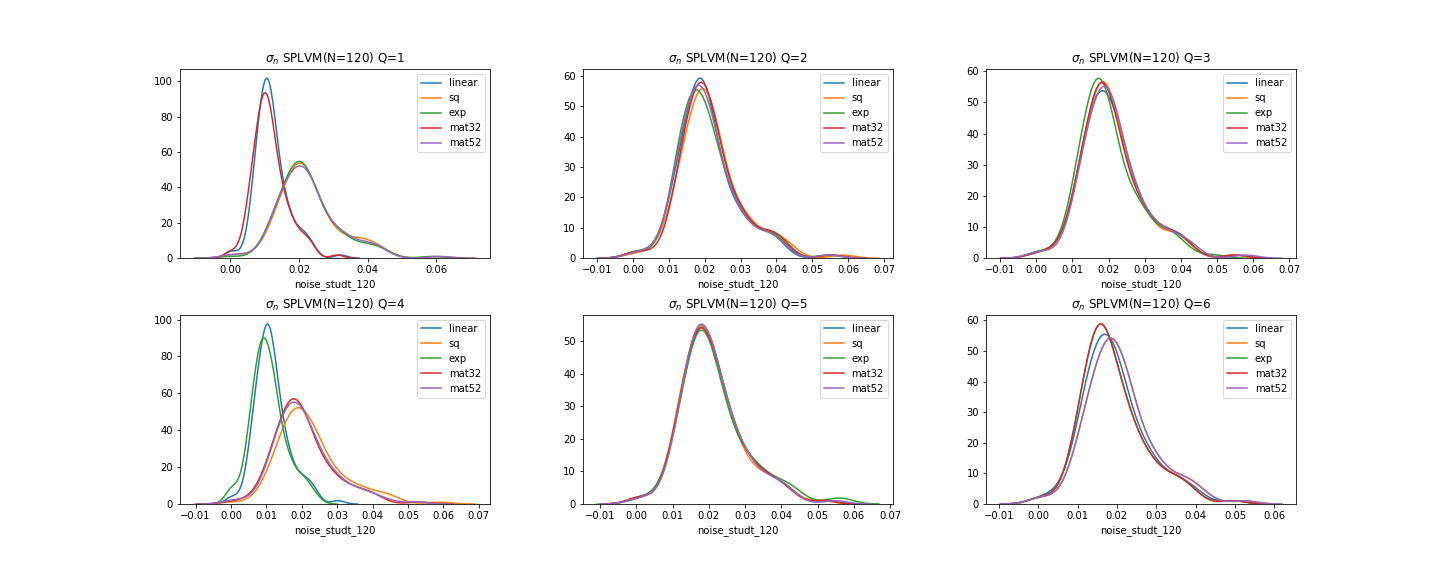
\includegraphics[width=7in]{img/07_1/noise_STUDT_120.png}
	\caption[SPLVM noise values for $N=120$, $D=754$]{The distributions of values of the vector $\sigma_n$. }
	\label{fig:studt_noises}
\end{figure}
\begin{figure}%fig:studt_variances
	\centering
	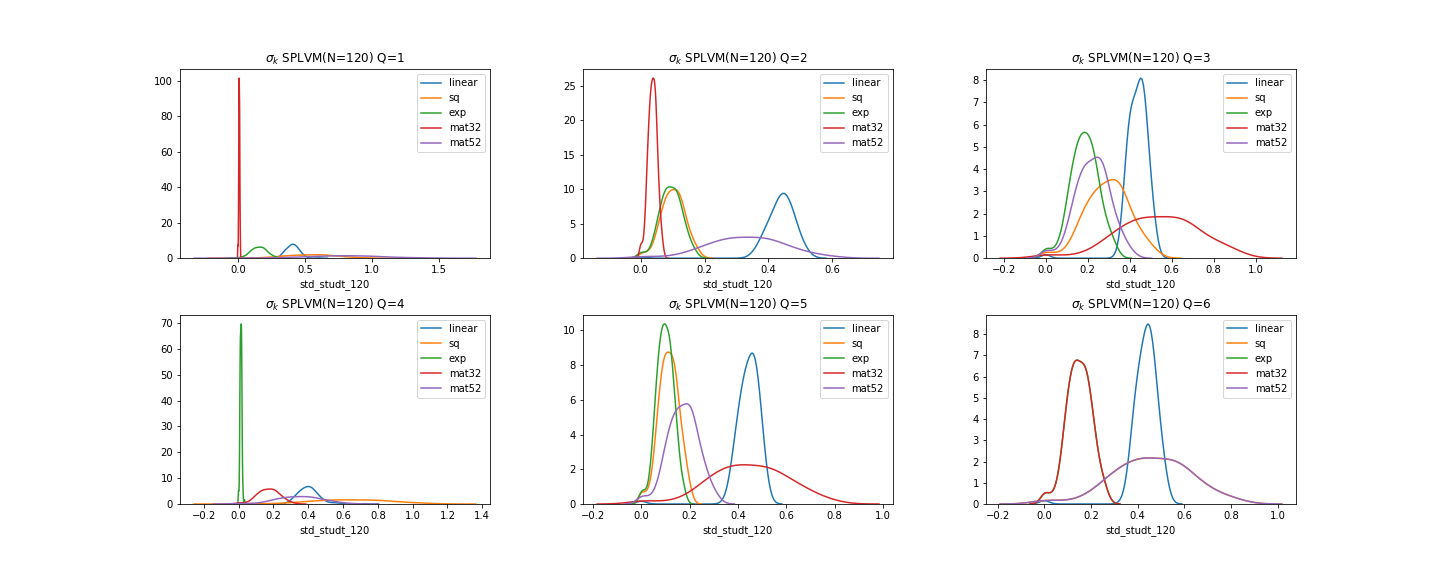
\includegraphics[width=7in]{img/07_1/std_STUDT_120.png}
	\caption[SPLVM variance values for $N=120$, $D=754$]{The distributions of values of the vector containing the variances.}
	\label{fig:studt_variances}
\end{figure}
The dependence of the SPLVM model on the size of data set was also determined by looking at different erroneous behaviors of reconstruction of the data, in figures \ref{fig:studt_N20_pairs}, \ref{fig:studt_N60_pairs}, \ref{fig:studt_N100_pairs} and \ref{fig:studt_N120_pairs}. Overall we observe that the systematic error observed in the GPLVM model results is lessened by applying the Student-t model to the same problem. 
\begin{figure}%fig:gplvm_N20_pairs
	\centering
	\begin{subfigure}[l]{0.3\textwidth}
		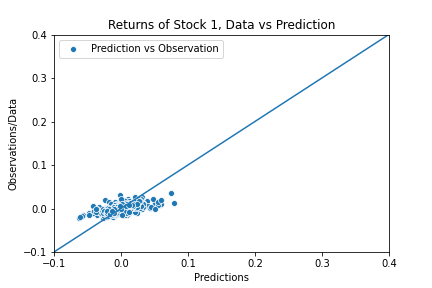
\includegraphics[width=\textwidth]{img/07_1/N20/Q1_kernel1_stock1_scatter.png}
	\end{subfigure}
	\begin{subfigure}[c]{0.3\textwidth}
		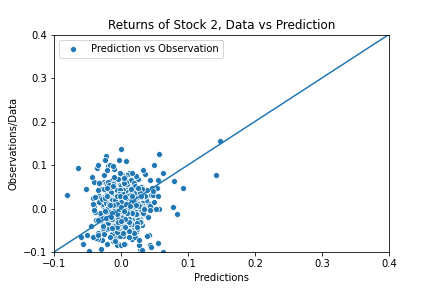
\includegraphics[width=\textwidth]{img/07_1/N20/Q1_kernel1_stock2_scatter.png}
	\end{subfigure}
	\begin{subfigure}[r]{0.3\textwidth}
		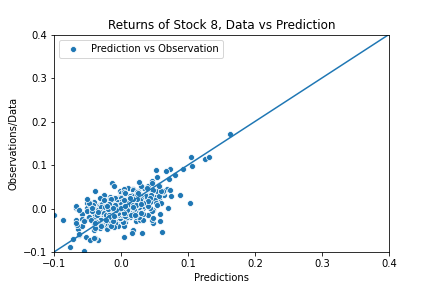
\includegraphics[width=\textwidth]{img/07_1/N20/Q1_kernel1_stock8_scatter.png}
	\end{subfigure}
	\caption[Y-$\hat{Y}$ pair plots for N=20 with the SPLVM model]{Plots from the SPLVM reconstruction with the $N=20$, $D=754$ dataset. The reconstruction failed showing the circular correct reconstruction of a 1D representation of the distribution of data points.}
	\label{fig:studt_N20_pairs}
\end{figure}
\begin{figure}%fig:gplvm_N60_pairs
	\centering
	\begin{subfigure}[l]{0.3\textwidth}
		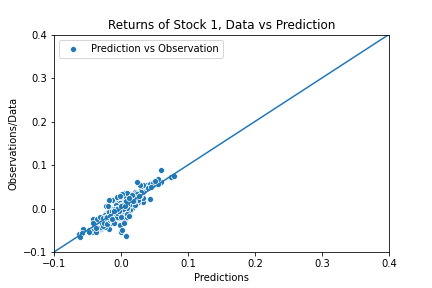
\includegraphics[width=\textwidth]{img/07_1/N60/Q1_kernel1_stock1_scatter.png}
	\end{subfigure}
	\begin{subfigure}[c]{0.3\textwidth}
		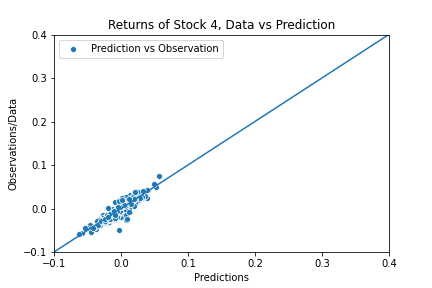
\includegraphics[width=\textwidth]{img/07_1/N60/Q1_kernel1_stock4_scatter.png}
	\end{subfigure}
	\begin{subfigure}[r]{0.3\textwidth}
		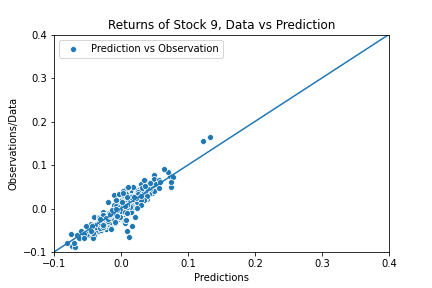
\includegraphics[width=\textwidth]{img/07_1/N60/Q1_kernel1_stock9_scatter.png}
	\end{subfigure}
	\caption[Y-$\hat{Y}$ pair plots for N=60 with the SPLVM model]{Plots from the SPLVM reconstruction with the $N=60$, $D=754$ dataset. The reconstruction worked properly. }
	\label{fig:studt_N60_pairs}
\end{figure}
\begin{figure}%fig:gplvm_N100_pairs
	\centering
	\begin{subfigure}[l]{0.3\textwidth}
		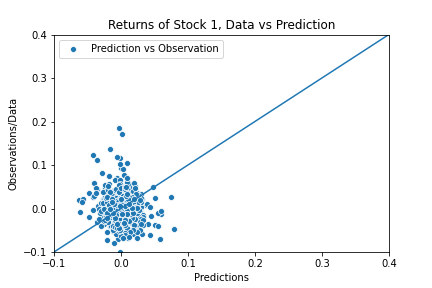
\includegraphics[width=\textwidth]{img/07_1/N100/Q1_kernel1_stock1_scatter.png}
	\end{subfigure}
	\begin{subfigure}[c]{0.3\textwidth}
		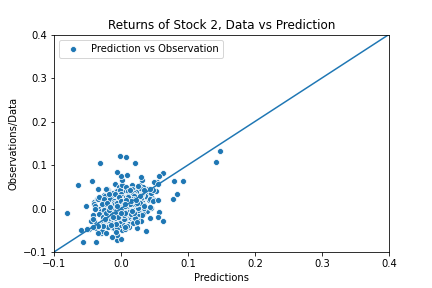
\includegraphics[width=\textwidth]{img/07_1/N100/Q1_kernel1_stock2_scatter.png}
	\end{subfigure}
	\begin{subfigure}[r]{0.3\textwidth}
		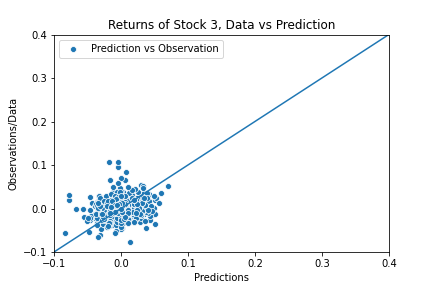
\includegraphics[width=\textwidth]{img/07_1/N100/Q1_kernel1_stock3_scatter.png}
	\end{subfigure}
	\caption[Y-$\hat{Y}$ pair plots for N=100 with the SPLVM model]{Plots from the SPLVM reconstruction with the $N=60$, $D=754$ dataset. The circular shape of the cloud indicates that the distributions of $Y$ and $\hat{Y}$ are well fit, but subpar reconstruction of the data has taken place.}
	\label{fig:studt_N100_pairs}
\end{figure}
\begin{figure}%fig:gplvm_N120_pairs
	\centering
	\begin{subfigure}[l]{0.3\textwidth}
		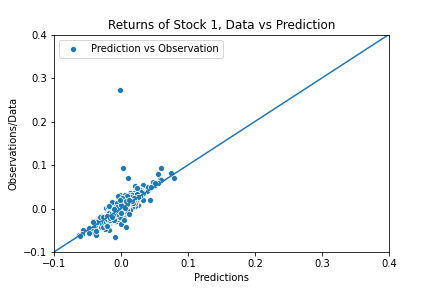
\includegraphics[width=\textwidth]{img/07_1/N120/Q1_kernel1_stock1_scatter.png}
	\end{subfigure}
	\begin{subfigure}[c]{0.3\textwidth}
		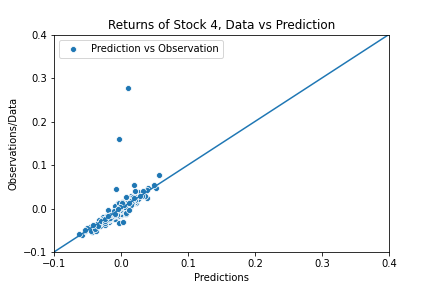
\includegraphics[width=\textwidth]{img/07_1/N120/Q1_kernel1_stock4_scatter.png}
	\end{subfigure}
	\begin{subfigure}[r]{0.3\textwidth}
		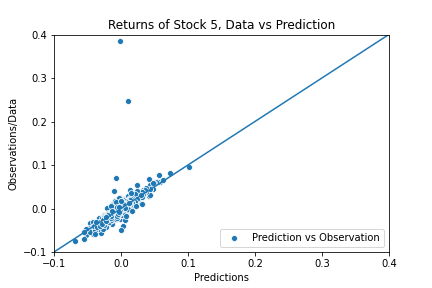
\includegraphics[width=\textwidth]{img/07_1/N120/Q1_kernel1_stock5_scatter.png}
	\end{subfigure}
	\caption[Y-$\hat{Y}$ pair plots for N=120 with the SPLVM model]{Plots from the SPLVM reconstruction with the $N=60$, $D=754$ dataset. We can find a good estimation of the true posterior, and a good reconstruction, while the off-diagonal that was observed with the GPLVM model is sufficiently smaller. }
	\label{fig:studt_N120_pairs}
\end{figure} 